\documentclass{standalone}
\usepackage{tikz}
\usepackage{nono}
\begin{document}
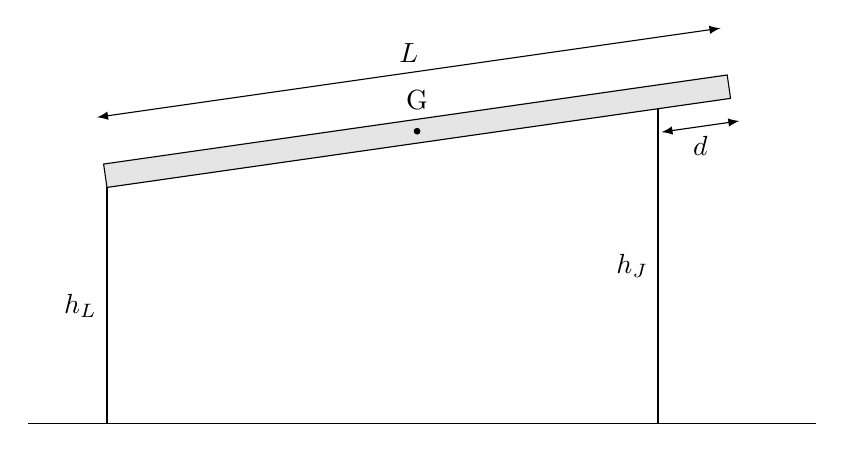
\begin{tikzpicture}
  \draw (0, 0) -- (10,0);
  \draw[thick] (1, 0) -- ++(0,3) coordinate(L) node[midway, left]{$h_L$}; 
  \draw[thick] (8, 0) -- ++(0,4) coordinate(J) node[midway, left]{$h_J$}; 
  \begin{scope}[rotate around={{atan(1/7)}:(1,3)}]
    \draw[fill=gray!20] (L) rectangle ++(8,0.3);
    \draw[fill=black] (L) ++(4, 0.15) coordinate (G) circle(1pt) node[above=0.15cm]{G};
    \draw[latex-latex] (J) ++(0, -0.3) -- ++(1,0) node[midway, below]{$d$};
    \draw[latex-latex] (L) ++(0, 0.9) -- ++(8,0) node[midway, above]{$L$};
  \end{scope}
\end{tikzpicture}
\end{document}
